\section{Introduction}
% \subsection{The Background and Importance of Open Source Projects}
% -- about open source communities in general
% -- importance of open source projects, maybe mention how flash died out, and the recent unity price change ?

% todo NN - il faudrait des éléments visuels qui illustre mais aussi donne à voir ce qu’est Processing, et éventuellement là “où est la communauté”: des screenshots de forums, etc.

\subsection{The Processing Project: A brief overview}
% todo - adapt to focus more on the research question

Processing was developed as a programming language and environment specifically tailored for the media arts communities. Its inception took place at the MIT Media Lab's Aesthetics and Computation Group (ACG) in 2001, led by Ben Fry and Casey Reas. Its foundational concepts build upon the earlier work from the Design By Numbers (DBN) programming platform, a project spearheaded by John Maeda \parencite{fryModernPrometheusHistory2018}.

Ben Fry shed light on the holistic nature of the Processing initiative, noting:
\begin{quote}
"The processing project is a community, a piece of software that you run, and a language. And that order is important." – Ben Fry \parencite[19:22]{artsatmit2017CASTSymposium2017}
\end{quote}

In its design philosophy, Processing introduced the concept of "software sketches". It was designed with an accessible entry point for beginners, while also providing advanced capabilities for experienced users \parencite{reasProcessingProgrammingMedia2006}.

Over the years, Processing has been adopted across various disciplines, showcasing its versatility. To further its impact and development, the Processing Foundation was established, with notable contributors like Daniel Shiffman. The foundation aims to support and expand the reach of the Processing software and its associated projects.

% todo add
%\subsection{Objective and Scope of the Research}

% Choice of processing, because the community has been around for a while and the project is still alive and taught in schools, also at a high school level

% modular toolkit, not a monolith
% community, application, syntax
% commercial software


    

\begin{figure}
  \centering
  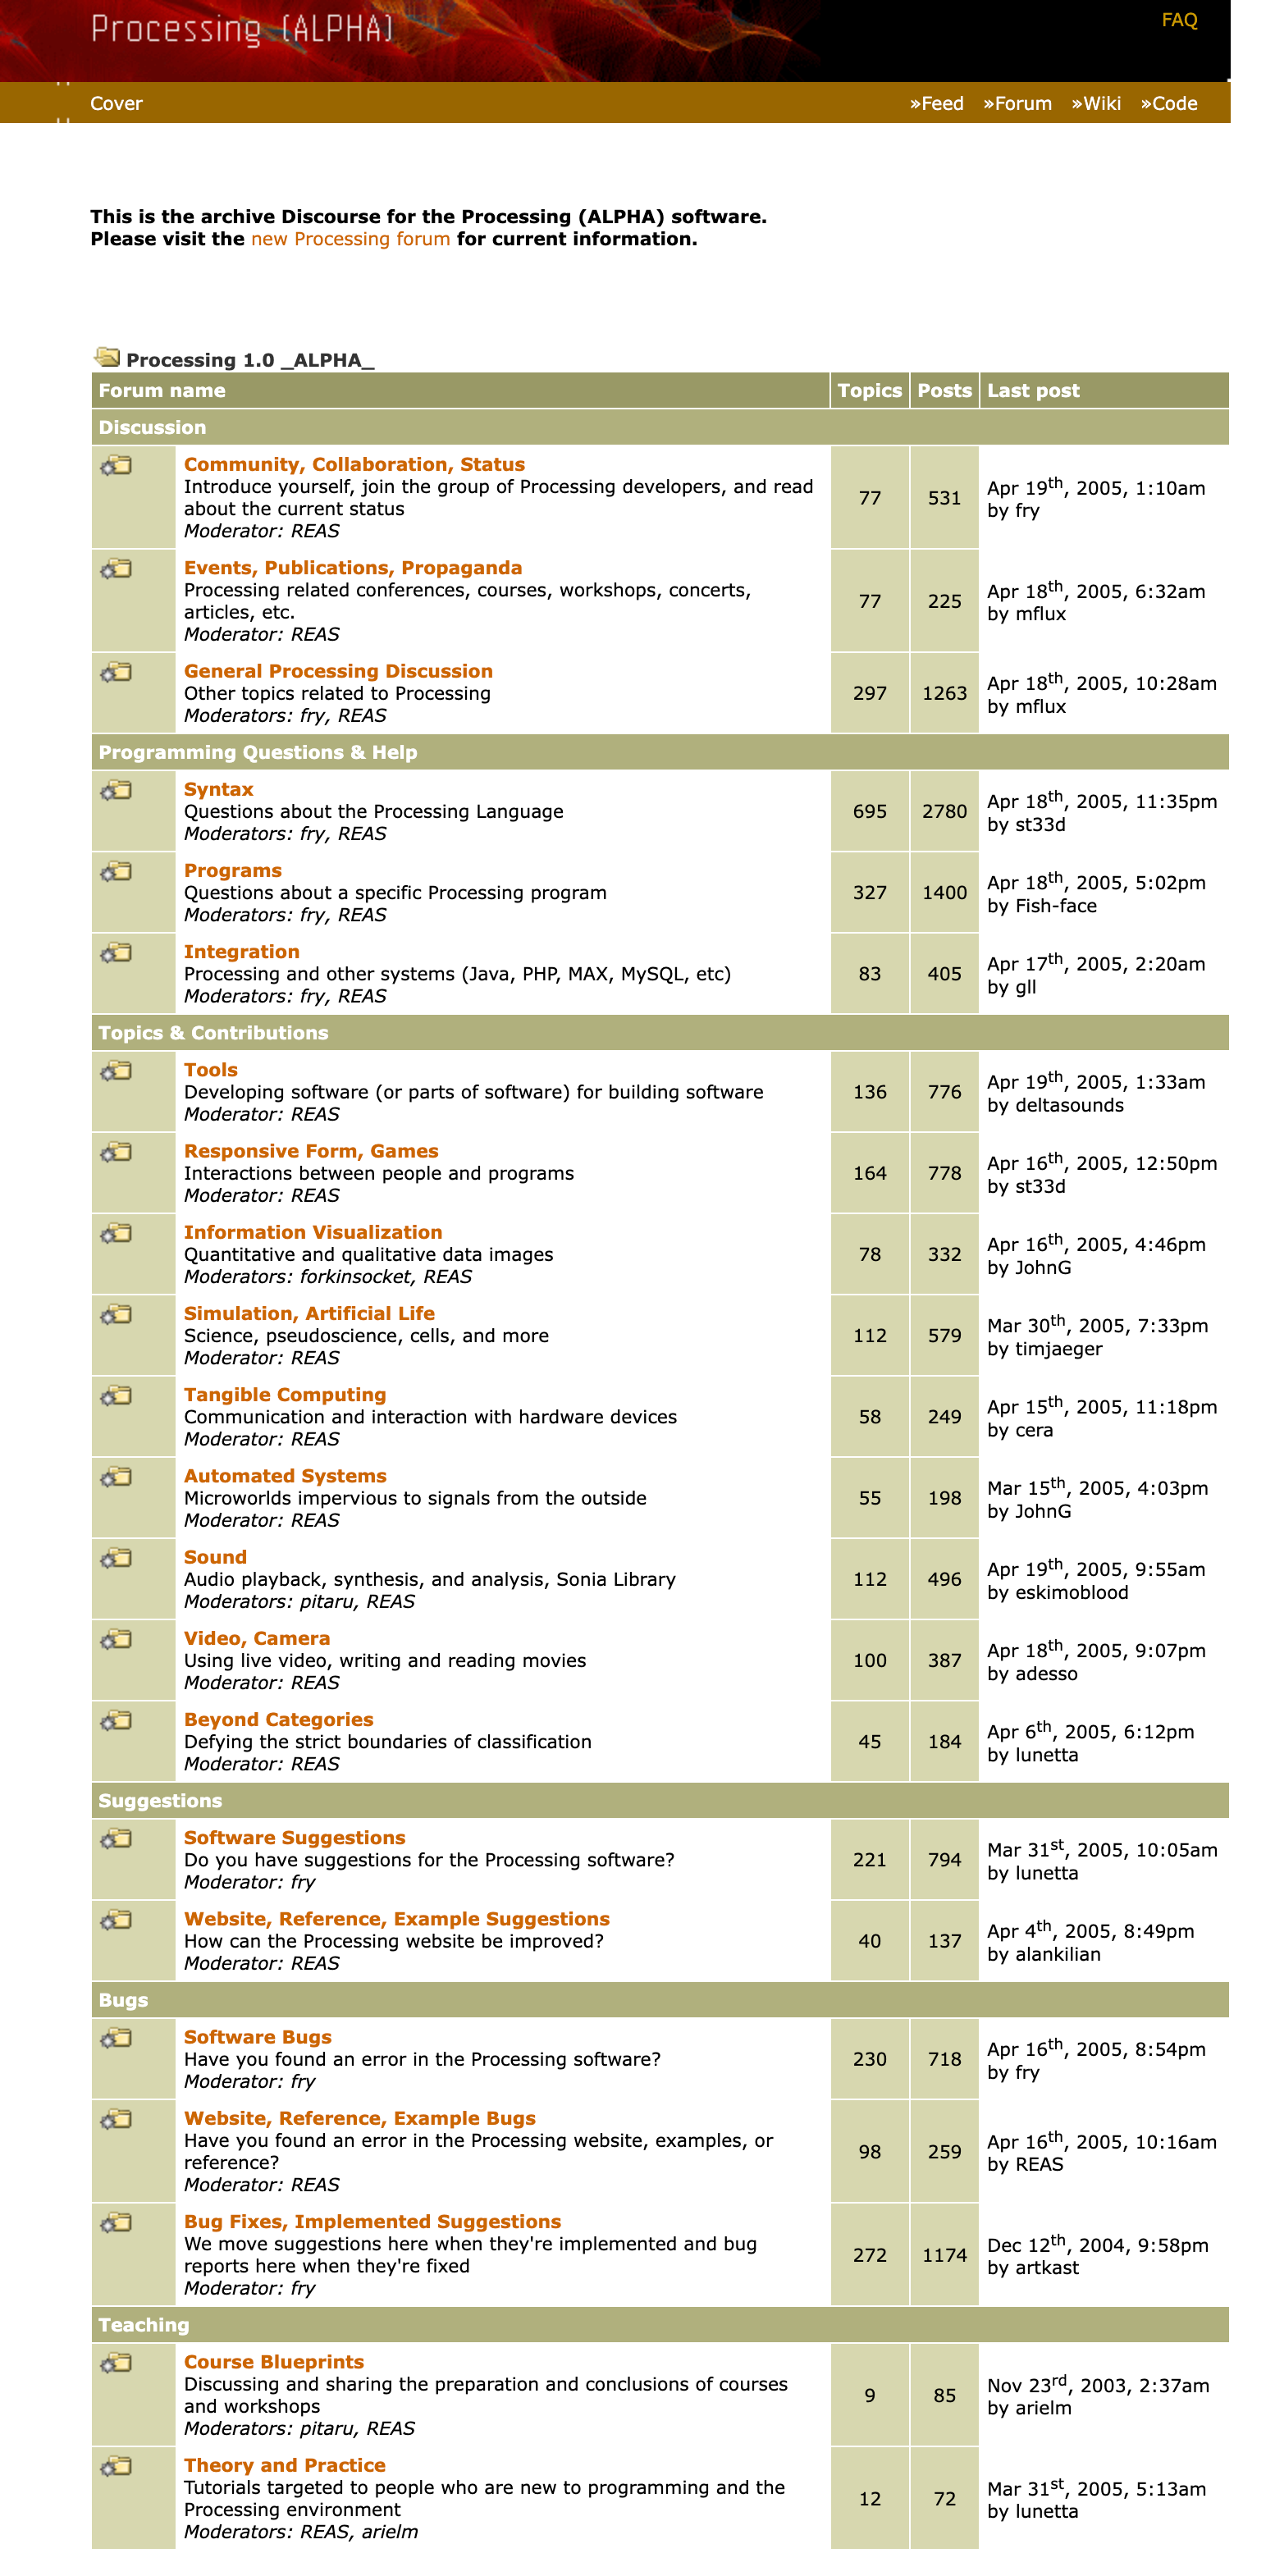
\includegraphics[width=0.7\textwidth]{images/processing_alpha_forum_screenshot.png} 
  \caption{Processing Alpha Forum (https://forum.processing.org/alpha)}
  \label{fig:alpha_forum_screenshot}
\end{figure}


\begin{figure}
  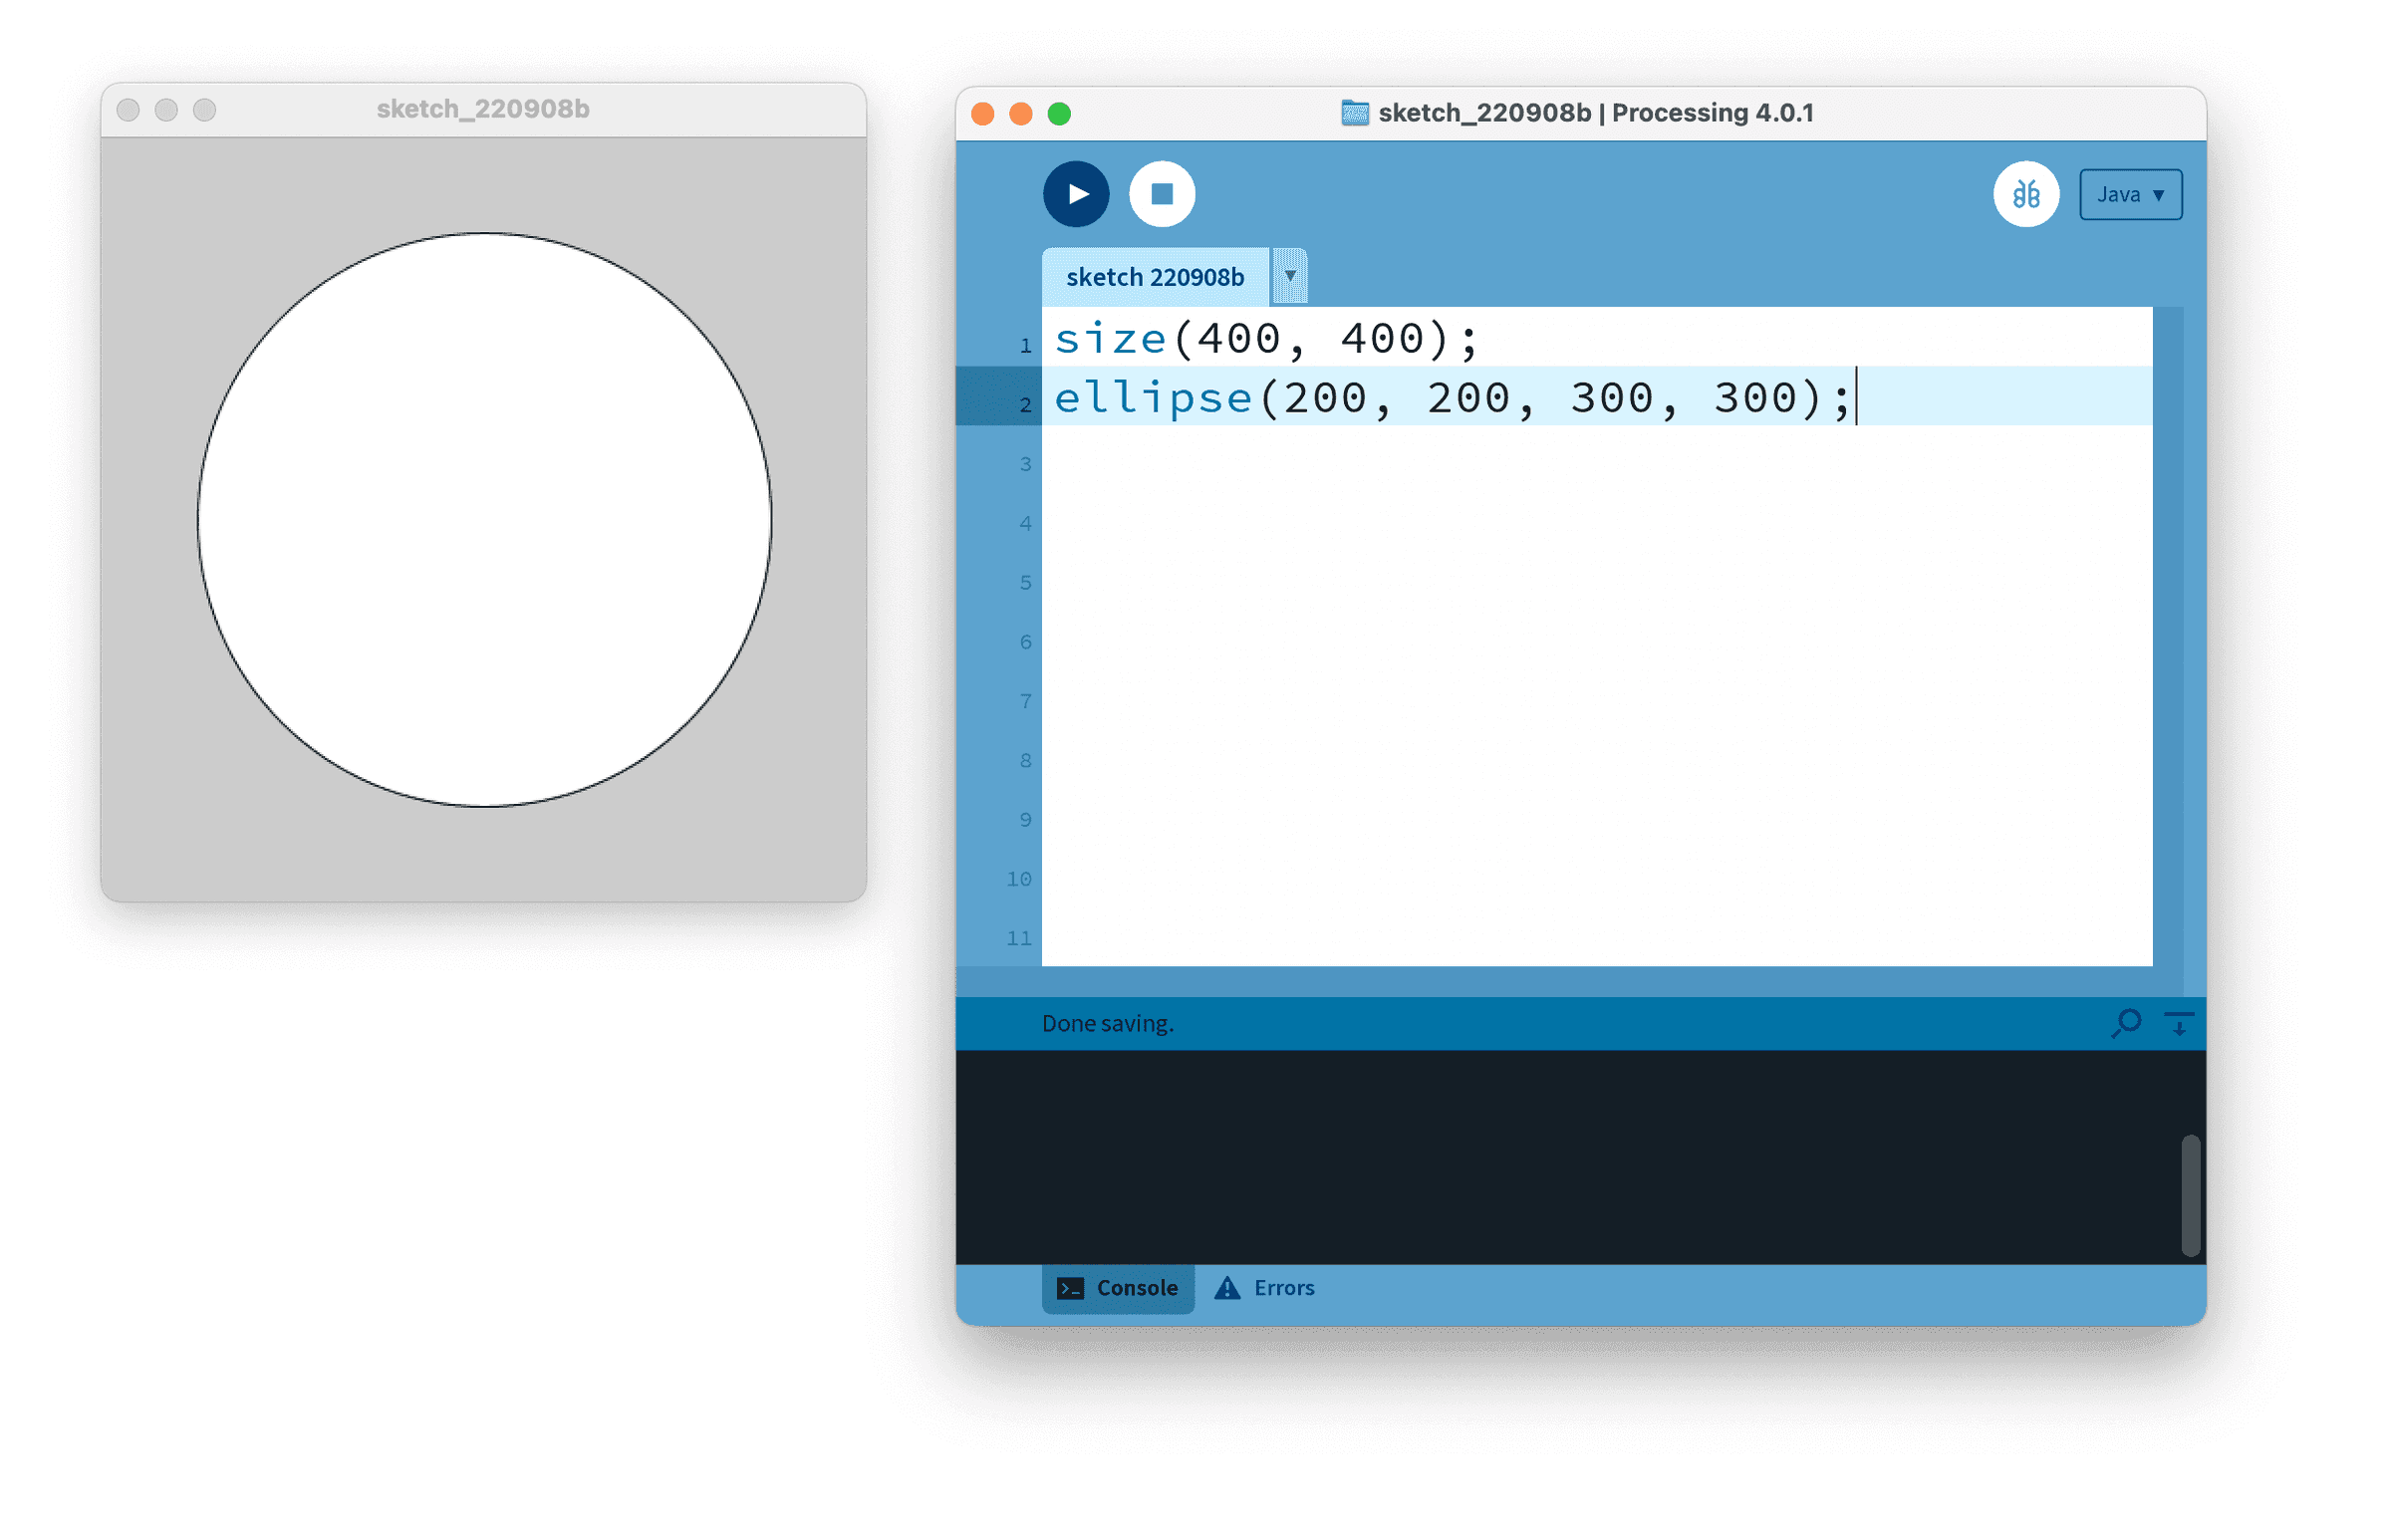
\includegraphics[width=0.5\textwidth]{images/processing_ide.png} 
  \caption{Processing IDE \parencite{reasProcessingIDE2015}}
  \label{fig:processing_ide_screenshot}
\end{figure}

% todo NN add figure about processing ide
% todo NN ne pas distinguer la litt review de l’introduction, ni la méthodo, il faudrait tout mettre dedans pour montrer (1) en quoi cela permet de formuler une question de recherche (qui reste à expliciter ici), (2) mettre en place une méthodologie pour y répondre

% todo NN Rappelle toi qu’une revue de littérature sert à préciser ton questionnement général décrcit en introduction et formuler une question de recherche puis une méthodo pour y répondre. Tu le fais heureusement déjà un peu !

% todo NN et en fin de cette grosses introduction tu pourrais mettre l’annonce du plan du mémoire, ce que vont contenir les chapitres

\section{Literature review}

\subsection{Open Source Contributions: Historical Perspective and Modern Implications}

Open source software has evolved from a grassroots, community-driven activity into a mainstream phenomenon influencing all sectors of software development. This transition has been analyzed from numerous perspectives, including Etienne Wenger's theory of Communities of Practice, which posits that learning occurs in social contexts \parencite{wengerCommunitiesPracticeLearning1998}. This theory underscores the importance of shared experiences, tools, and discourse in shaping a community's collective practice. In the context of open-source software, these dynamics offer invaluable insights into the sustainability and progression of such projects. For instance, the Processing community exemplifies more than just a collection of individual contributors; it represents a dynamic community molded by common goals and collective learning.

This communal focus contrasts sharply with the software development models described in Eric S. Raymond's seminal work "The Cathedral and the Bazaar" \parencite{CathedralBazaarMusings2002a}. The Cathedral model is marked by careful planning and centralized authority, more akin to the early GNU projects initiated by Richard Stallman in the 1980s. Conversely, the Bazaar model encourages open collaboration and decentralization—features commonly associated with contemporary open source projects. These two models can be conceptualized as endpoints of a continuum, with real-world communities of practice, like the Processing community, potentially embodying characteristics of both.

Although Richard Stallman's Free Software Movement initially utilized a Cathedral-like approach, the evolution of version control systems like Git has facilitated the adoption of more decentralized, Bazaar-like models. This technological and philosophical shift intriguingly complements Wenger's notions of "mutual engagement," "joint enterprise," and "shared repertoire"—elements that nurture a sense of community and shared objectives \parencite{wengerCommunitiesPracticeLearning1998}.

Fast-forwarding to today, the landscape now includes not just individual contributors but major corporations as well, injecting both challenges and opportunities into existing communities. The Processing project stands as a compelling case study to examine how an open-source community can preserve its foundational ethos while simultaneously adapting to contemporary requirements.

To holistically grasp the intricate interplay of social and technical factors contributing to the success of open-source initiatives, a multidimensional analysis is essential. Such an approach would synthesize various frameworks, including Wenger's Communities of Practice \parencite{wengerCommunitiesPracticeLearning1998} and Raymond's Cathedral and Bazaar models \parencite{CathedralBazaarMusings2002a}, aiming to provide a nuanced understanding of a community's past, present dynamics, and future potential.




\subsection{The Centrality of Open Source Values in Processing}

% Contextualizing the Open Source Movement
The open source movement has undeniably influenced a myriad of practical applications, ranging from operating systems like Linux to various software tools. However, its impact on the realm of creative software tools has been comparatively limited. According to Reas and Fry~\parencite[30]{reasProcessingProgrammingHandbook2007}, companies like Adobe and Microsoft largely dominate the field, limiting the open-source philosophy's penetration into the culture of arts software. % Here, you establish the broader impact of open source and point out a gap in its influence over artistic software.

% Importance of Open Source Ethos in Processing
Within this context, Processing emerges as a significant counterexample, embedding the ethos of open source at its very core. This ethos is not simply a byproduct but an intentional design choice to promote software literacy. Reas and Fry define literacy in the context of software as the ability to both "read" and "write" within a medium~\parencite[29]{reasProcessingProgrammingHandbook2007}. % This highlights how Processing intentionally incorporates open source values to facilitate a specific kind of literacy.

% Elaborating Software Literacy
In traditional print writing, literacy involves generating rhetorical tools that aim to demonstrate and convince. In contrast, computer-based literacy enables one to create processes that can simulate and decide. % This part elaborates on what software literacy entails, contrasting it with traditional forms of literacy.

% Processing's Alignment with Design Principles
Moreover, Processing exemplifies many of the Design Principles for Tools to Support Creative Thinking as suggested by Resnick~\parencite{resnickDesignPrinciplesTools}. Particularly, by fostering a culture of collaboration and open exchange, Processing does not merely align with open source motivations but elevates itself as a superior Creativity Support Tool (CST). % This wraps up the section by connecting Processing's open-source ethos to broader design principles, emphasizing its role as a potent CST.




\subsection{Understanding the Drivers of Open Source Contributions in the Processing Community}

While existing literature often focuses on the role of companies in contributing to open-source projects through complementary services like consulting, our study diverges by focusing on individual contributors. In the context of the Processing community, corporate involvement is notably lesser when compared to platforms like Linux that have substantial corporate contributions.

The 2016 Processing community survey revealed a significant number of users employ the language for educational purposes. This is consistent with Processing's design ethos, which is aimed at being educationally accessible. However, the extent to which this educational usage intersects with what can be termed as `professional use' remains unclear.

For the purpose of this study, `professional use' is understood to primarily include artists and designers. This nuanced categorization helps in probing the overlap between professional and educational use within the Processing community.

Building upon established frameworks such as the taxonomy by Bonaccorsi et al.~\cite{bonaccorsiComparingMotivationsIndividual2006}, which categorizes motivations behind open-source contributions into Economic, Social, and Technological domains, our study intends to adapt this taxonomy to suit the specific nuances of the Processing community.

\begin{figure}[h!] 
  \centering
  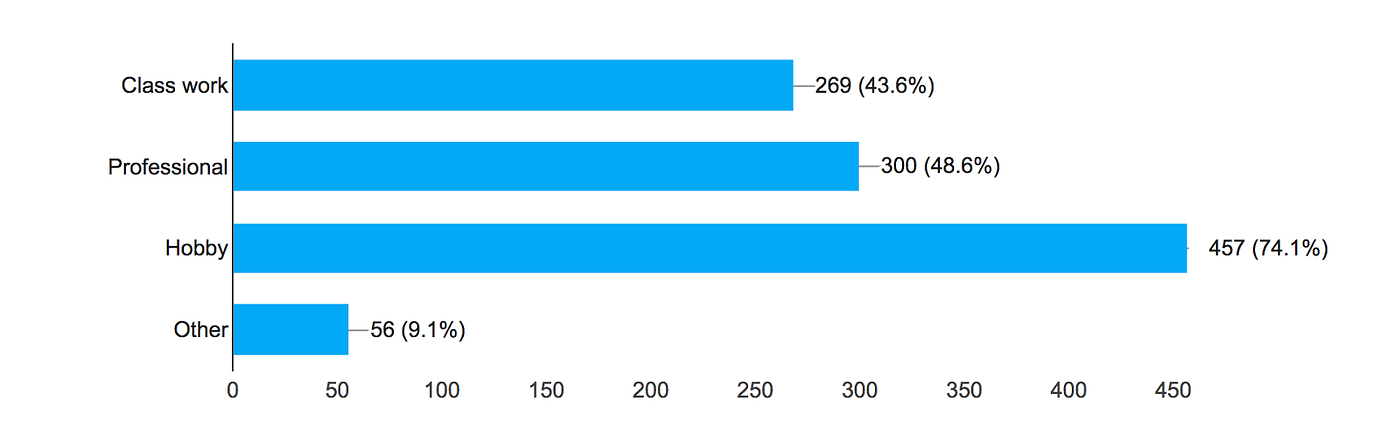
\includegraphics[width=0.9\textwidth]{images/community-survey.png} 
  \caption{Processing 2016 community survey result \parencite{2016CommunitySurvey}}
  \label{fig:community_survey}
\end{figure}

\begin{table}
    \begin{tabularx}{\textwidth}{l X} % X is a placeholder for stretching the column
    \toprule
    Motivation area & Micro level \\
    \midrule
    Economic & Monetary rewards \\
     & Low opportunity costs \\
     & Gaining a reputation among peers \\
     & Gaining future career benefits \\
    \midrule
    Social & Fun to program (Loving to code) \\
     & Altruism (gift economy) \\
     & Sense of belonging to the community \\
     & Fight against proprietary software \\
    \midrule
    Technological & Learning \\
     & Contributions and feedback from the community \\
     & Working with a bleeding-edge technology \\
     & Scratching a personal itch \\
    \bottomrule
    \end{tabularx} % End of tabularx environment
    \label{tab:taxonomy}
    \caption{Taxonomy of Individual Programmers’ Motivations. Adapted from \parencite{bonaccorsiComparingMotivationsIndividual2006}}

\end{table}

% todo NN cette taxonomie est intéressante, mais il faudrait la commenter dans le corps de texte en 2.2, qu’elle vienne nourrir ce que tu as mis au-dessus comme texte, là tu la pose rapidement sans trop détailler comment elle a été produite et ce qu’elle nous dit

%\subsection{The intersection of Creative Coding and Open Source}
%\subsection{Relevant Methodological Approaches in Computer Science and Anthropology}
